\documentclass[11pt,a4paper]{article}

\usepackage[margin=2.0cm]{geometry}
\usepackage{amsmath,amssymb,amsfonts}
\usepackage[T1]{fontenc}
\usepackage{lmodern}
\usepackage{microtype}
\usepackage{enumitem}
\usepackage{booktabs}
\usepackage{tabularx}
\usepackage{xcolor}
\usepackage[hidelinks,colorlinks=true,
            urlcolor=blue!50!black,
            linkcolor=blue!50!black]{hyperref}
\usepackage{listings}
\usepackage{tikz}
\usepackage{pgfplots}
\pgfplotsset{compat=1.18}
\usetikzlibrary{positioning,arrows.meta,shapes.geometric,fit,calc,
                decorations.pathreplacing,backgrounds}

\definecolor{matclr}{RGB}{40,103,160}
\definecolor{unitclr}{RGB}{180,70,40}
\definecolor{rawclr}{RGB}{50,140,80}
\definecolor{prodclr}{RGB}{160,60,140}
\definecolor{kept}{RGB}{40,140,80}
\definecolor{cut}{RGB}{170,60,60}
\definecolor{accent}{RGB}{200,120,30}
\definecolor{capex}{RGB}{40,103,160}
\definecolor{opex}{RGB}{120,120,120}
\definecolor{co2}{RGB}{170,60,60}
\definecolor{h2o}{RGB}{40,140,180}

\tikzset{
  mat/.style={circle,draw=matclr,thick,fill=matclr!10,
              minimum size=7mm,inner sep=0.5pt,font=\scriptsize},
  raw/.style={mat,draw=rawclr,fill=rawclr!12},
  prod/.style={mat,draw=prodclr,fill=prodclr!12,line width=0.5mm},
  unit/.style={rectangle,draw=unitclr,thick,fill=unitclr!10,
                minimum height=6mm,minimum width=14mm,
                rounded corners=1pt,inner sep=1pt,font=\scriptsize},
  unitin/.style={unit,fill=kept!18,draw=kept!80},
  unitout/.style={unit,fill=cut!12,draw=cut!60,opacity=0.5},
  edge/.style={-{Stealth[length=1.6mm]},semithick},
}

\lstset{
  basicstyle=\ttfamily\footnotesize,
  breaklines=true, columns=fullflexible, keepspaces=true,
  showstringspaces=false, frame=single, rulecolor=\color{gray!30},
}

\newcommand{\HyMeKo}{\textsc{HyMeKo}}
\newcommand{\code}[1]{\texttt{\small #1}}
\setlist[itemize]{leftmargin=1.4em,itemsep=2pt,topsep=3pt}
\setlist[enumerate]{leftmargin=1.6em,itemsep=2pt,topsep=3pt}

\title{P-graph multi-objective ABB in $\HyMeKo$\\[2pt]
       \large\normalfont four structurally distinct methanol-synthesis
       plants from one DSL and four weight vectors}
\author{For Jean Pimentel (Pannonia / P-graph community)}
\date{2026-05-19 (Stage P-mo)}

\begin{document}
\maketitle

\begin{center}
\fbox{\begin{minipage}{0.92\linewidth}\small
\textbf{In one sentence.} The Friedler--Tarj\'an--Huang--Fan 1992 ABB
generalises from the single-criterion cost interface
$c: O \to \mathbb{R}_{\geq 0}$ to a weighted-sum form
$c_{\boldsymbol{w}}(u) = \langle\boldsymbol{w}, \boldsymbol{c}(u)\rangle$
without modifying the bound machinery, because both the inclusion bound
(cost monotone-non-decreasing) and the reachability bound (structural)
survive intact under non-negative weights and cost vectors. We provide a
reference Rust implementation in $\HyMeKo$/\texttt{hymeko\_pgraph},
demonstrated on an $11$-unit methanol-synthesis worked example with
$4$-dimensional costs (CAPEX, OPEX, CO$_2$, H$_2$O). Five weight
regimes produce \textbf{four structurally distinct optimal plants},
including a non-obvious hybrid topology (cheap flue-gas CO$_2$ capture
$+$ green-H$_2$ electrolysis) that neither single-criterion regime
selects on its own.
\end{minipage}}
\end{center}

\vspace{4pt}

% ===================================================================
\section{The objective and the bound}

The scalar-cost ABB (Friedler 1992) minimises $\sum_{u \in O'} c(u)$
over feasible structures $O' \subseteq O_{\max}$. Stage P-mo extends
the per-unit cost to a $D$-dimensional vector
$\boldsymbol{c}(u) \in \mathbb{R}_{\geq 0}^D$ across named dimensions
(\textsc{capex}, \textsc{opex}, \textsc{co}$_2$, \textsc{h}$_2$o, $\ldots$)
and accepts a user weight vector
$\boldsymbol{w} \in \mathbb{R}_{\geq 0}^D$. The objective becomes
\[
\boxed{\;\min_{O' \subseteq O_{\max}}\;
  \sum_{u \in O'} \bigl\langle\boldsymbol{w}, \boldsymbol{c}(u)\bigr\rangle
  \;=\;
  \sum_{u \in O'}\sum_{d=1}^{D} w_d \cdot c_d(u)\;}
\]
subject to the unchanged feasibility constraints (input consistency,
demand, strict no-excess by default).

\paragraph{Admissibility preservation.}
\begin{itemize}
\item Inclusion bound: since $w_d \geq 0$ and $c_d(u) \geq 0$, every
      inclusion adds a non-negative term, so the partial-cost is a
      lower bound on the descendant's full cost. Prune when
      partial $\geq$ incumbent.
\item Reachability bound: structural ($C_R(\widehat{O}) \supseteq P$),
      not cost-based. Unaffected by the weighting.
\end{itemize}

The bound machinery is bytes-for-bytes the original Friedler '92.
Only the per-unit cost evaluation is generalised --- everywhere
the old code called \code{p.costs.get(\&u)} the new code calls
\code{effective\_cost(p, opts, u)}, which branches on
\code{opts.cost\_weights}: \code{None} returns the scalar cost
(byte-identical to pre-P-mo), \code{Some(w)} returns the dot
product.

% ===================================================================
\section{The methanol-synthesis worked example}

\subsection{Process and \HyMeKo{} encoding}

CO$_2$ $+$ H$_2$ $\to$ CH$_3$OH $+$ H$_2$O. The plant catalogue
contains 11 operating units organised as two binary forks plus an
obligated downstream finishing chain:

\begin{itemize}[itemsep=1pt]
\item \textbf{CO$_2$ source}: \code{CaptureFlue} (cheap CAPEX,
      moderate CO$_2$) vs \code{CaptureDAC} (high CAPEX, low
      CO$_2$, high H$_2$O).
\item \textbf{H$_2$ route}: \code{SMR} (cheap CAPEX, huge CO$_2$)
      vs \code{Electrolyzer} (high CAPEX, low CO$_2$, very high
      H$_2$O).
\item \textbf{Mixer-after-H$_2$}: structurally forced
      (\code{MixerBlue} after SMR, \code{MixerGreen} after
      Electrolyzer).
\item \textbf{Downstream chain}: \code{MeOHReactor} $\to$
      \code{Distillation} $\to$ product; \code{WaterTreatment}
      and \code{SteamRecycle} as no-product consumers of
      reactor by-products (required by strict no-excess).
\end{itemize}

The four-dimensional cost annotations are written with
$\HyMeKo$'s existing tagged-child-node grammar; no parser
extension is required:

\begin{lstlisting}
@MeOHReactor <unit> 1100 {
    cost <capex> 1100;
    cost <opex>   260;
    cost <co2>     22;
    cost <h2o>     14;
    (-syngas, +crude_methanol, +waste_water);
}
\end{lstlisting}

\subsection{The full P-graph}

\begin{center}
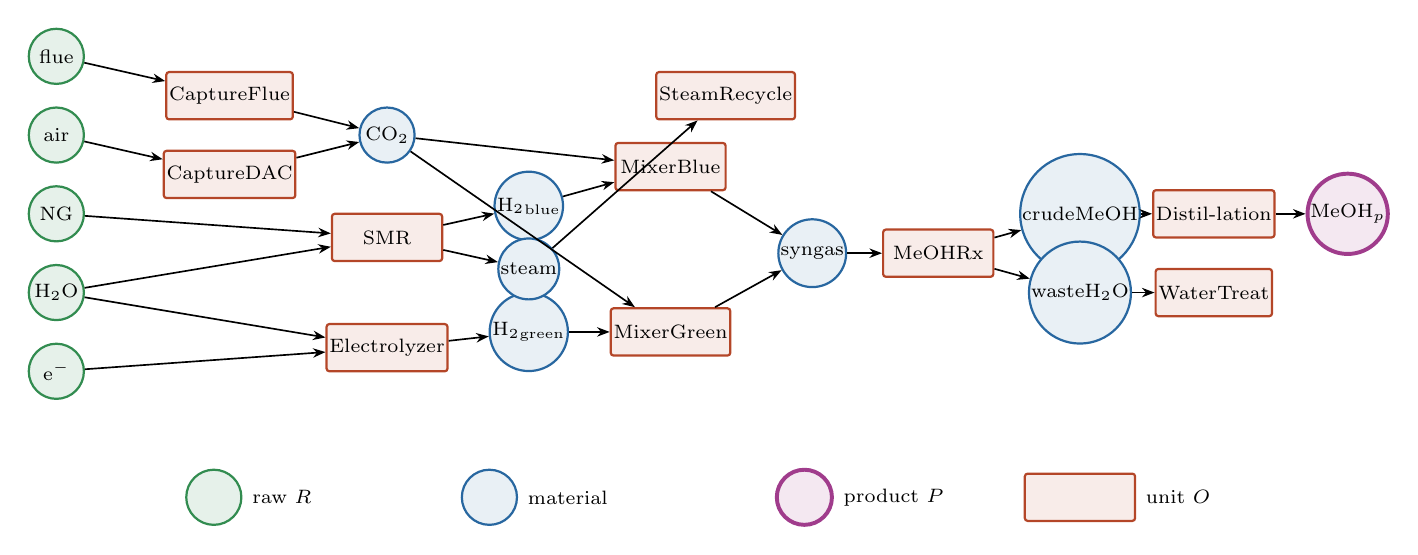
\begin{tikzpicture}[node distance=4mm and 8mm]
% Raws (left column)
\node[raw] (flue) at (0,3.0) {flue};
\node[raw] (air)  at (0,2.0) {air};
\node[raw] (ng)   at (0,1.0) {NG};
\node[raw] (h2o_in) at (0,0.0) {H$_2$O};
\node[raw] (e)    at (0,-1.0) {e$^-$};

% Capture units
\node[unit] (capF) at (2.2, 2.5) {Capture\\Flue};
\node[unit] (capD) at (2.2, 1.5) {Capture\\DAC};

% CO2_pure intermediate
\node[mat]  (co2p) at (4.2, 2.0) {CO$_2$};

% H2 routes
\node[unit] (smr)  at (4.2, 0.7) {SMR};
\node[unit] (elec) at (4.2,-0.7) {Electro\\lyzer};

% H2 intermediates + steam
\node[mat] (h2b)   at (6.0, 1.1) {H$_2$\textsubscript{blue}};
\node[mat] (h2g)   at (6.0,-0.5) {H$_2$\textsubscript{green}};
\node[mat] (steam) at (6.0, 0.3) {steam};

% Mixers
\node[unit] (mixB) at (7.8, 1.6) {Mixer\\Blue};
\node[unit] (mixG) at (7.8,-0.5) {Mixer\\Green};

% Syngas
\node[mat] (syn)   at (9.6, 0.5) {syngas};

% Reactor + chain
\node[unit] (rx)   at (11.2, 0.5) {MeOH\\Rx};
\node[mat]  (cr)   at (13.0, 1.0) {crude\\MeOH};
\node[mat]  (ww)   at (13.0, 0.0) {waste\\H$_2$O};

\node[unit] (dist) at (14.7, 1.0) {Distil-\\lation};
\node[unit] (wt)   at (14.7, 0.0) {Water\\Treat};
\node[unit] (sr)   at (8.5, 2.5) {Steam\\Recycle};

\node[prod] (meoh) at (16.4, 1.0) {MeOH$_p$};

% Edges
\draw[edge] (flue) -- (capF);
\draw[edge] (air)  -- (capD);
\draw[edge] (capF) -- (co2p);
\draw[edge] (capD) -- (co2p);

\draw[edge] (ng)     -- (smr);
\draw[edge] (h2o_in) -- (smr);
\draw[edge] (smr)    -- (h2b);
\draw[edge] (smr)    -- (steam);

\draw[edge] (e)      -- (elec);
\draw[edge] (h2o_in) -- (elec);
\draw[edge] (elec)   -- (h2g);

\draw[edge] (co2p) -- (mixB);
\draw[edge] (h2b)  -- (mixB);
\draw[edge] (co2p) -- (mixG);
\draw[edge] (h2g)  -- (mixG);

\draw[edge] (mixB) -- (syn);
\draw[edge] (mixG) -- (syn);
\draw[edge] (syn)  -- (rx);
\draw[edge] (rx)   -- (cr);
\draw[edge] (rx)   -- (ww);

\draw[edge] (cr)   -- (dist);
\draw[edge] (ww)   -- (wt);
\draw[edge] (dist) -- (meoh);
\draw[edge] (steam) -- (sr);

% Legend (right side)
\begin{scope}[xshift=0cm, yshift=-2.6cm]
\node[raw,label=right:{\scriptsize raw $R$}]      at (2.0,0) {};
\node[mat,label=right:{\scriptsize material}]      at (5.5,0) {};
\node[prod,label=right:{\scriptsize product $P$}]  at (9.5,0) {};
\node[unit,label=right:{\scriptsize unit $O$}]     at (13.0,0) {};
\end{scope}

\end{tikzpicture}\\[2pt]
\small\textit{Figure 1.} The methanol-synthesis P-graph. Two binary forks
(CO$_2$ source and H$_2$ route) plus the obligated downstream chain.
The $2 \times 2$ choice space has $4$ topologically distinct routes;
ABB selects one (or a hybrid) under each weight vector.
\end{center}

\subsection{The cost table}

\begin{center}\small
\begin{tabular}{lrrrrr}
\toprule
Unit              & scalar    & CAPEX & OPEX & CO$_2$ & H$_2$O \\
\midrule
CaptureFlue       & 800       & 800   & 220  & 45     & 8 \\
CaptureDAC        & 1900      & 1900  & 180  & 12     & 35 \\
SMR               & 600       & 600   & 210  & \textbf{310}    & 12 \\
Electrolyzer      & 1400      & 1400  & 320  & 18     & \textbf{160} \\
MixerBlue / Green & 90        & 90    & 25   & 3      & 1 \\
MeOHReactor       & 1100      & 1100  & 260  & 22     & 14 \\
Distillation      & 350       & 350   & 140  & 9      & 22 \\
WaterTreatment    & 180       & 180   & 70   & 4      & 0 \\
SteamRecycle      & 60        & 60    & 30   & 1      & 0 \\
\bottomrule
\end{tabular}
\end{center}

The two highlighted entries are the engineering tradeoffs that drive
the structural decisions: \textbf{SMR is cheap but carbon-heavy};
\textbf{Electrolyzer is carbon-clean but water-hungry}.

% ===================================================================
\section{Five weight regimes, four structurally distinct optima}

We run the new \code{hymeko\_pgraph\_dump --weights ...} CLI against
the methanol-synthesis source under five weight vectors. The table:

\begin{center}\small
\begin{tabular}{lll r r}
\toprule
Regime & $\boldsymbol{w}$ (CAPEX, OPEX, CO$_2$, H$_2$O) & Optimal topology & wcost & nodes \\
\midrule
Scalar fallback     & ---                          & \texttt{CaptureFlue $+$ SMR $+$ MixerBlue} & 3180 & 173 \\
CAPEX-only          & $(1.0, 0, 0, 0)$             & same as scalar                            & 3180 & --- \\
\textbf{CO$_2$-heavy} & $(0.01, 0.01, 100, 0.01)$ & \texttt{CaptureDAC $+$ Electrolyzer $+$ MixerGreen} & 6862 & --- \\
\textbf{H$_2$O-heavy} & $(0.01, 0.01, 0.01, 100)$ & same as scalar (water punishes green)     & 5745 & --- \\
\textbf{Joint}      & $(1.0, 0.5, 10, 1.0)$        & \texttt{CaptureFlue $+$ Electrolyzer $+$ MixerGreen} & 5653 & --- \\
\bottomrule
\end{tabular}\\[3pt]
\small\textit{Table 1.} Five weight regimes. The wcost column gives the
weighted-sum cost achieved.
\end{center}

\subsection{The four optima as small-multiples}

\begin{center}
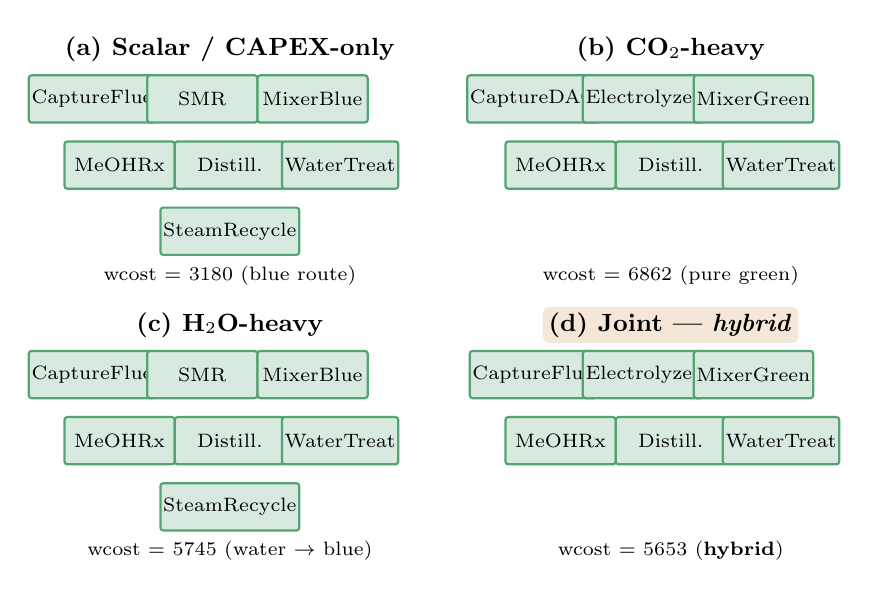
\begin{tikzpicture}[x=0.7cm, y=0.7cm]

% ── (a) Scalar / CAPEX-only — blue route
\begin{scope}[shift={(0,0)}]
\node[font=\small\bfseries] at (3.0, 3.3) {(a) Scalar / CAPEX-only};
\node[unitin] (cf1) at (0.5, 2.4) {CaptureFlue};
\node[unitin] (sm1) at (2.5, 2.4) {SMR};
\node[unitin] (mb1) at (4.5, 2.4) {MixerBlue};
\node[unitin] (rx1) at (1.0, 1.2) {MeOHRx};
\node[unitin] (di1) at (3.0, 1.2) {Distill.};
\node[unitin] (wt1) at (5.0, 1.2) {WaterTreat};
\node[unitin] (sr1) at (3.0, 0.0) {SteamRecycle};
\node[font=\scriptsize] at (3.0, -0.8) {wcost = 3180  (blue route)};
\end{scope}

% ── (b) CO2-heavy — pure green route
\begin{scope}[shift={(8,0)}]
\node[font=\small\bfseries] at (3.0, 3.3) {(b) CO$_2$-heavy};
\node[unitin] (cd2) at (0.5, 2.4) {CaptureDAC};
\node[unitin] (el2) at (2.5, 2.4) {Electrolyzer};
\node[unitin] (mg2) at (4.5, 2.4) {MixerGreen};
\node[unitin] (rx2) at (1.0, 1.2) {MeOHRx};
\node[unitin] (di2) at (3.0, 1.2) {Distill.};
\node[unitin] (wt2) at (5.0, 1.2) {WaterTreat};
\node[font=\scriptsize] at (3.0, -0.8) {wcost = 6862  (pure green)};
\end{scope}

% ── (c) H2O-heavy — same as scalar (water punishes green)
\begin{scope}[shift={(0,-5)}]
\node[font=\small\bfseries] at (3.0, 3.3) {(c) H$_2$O-heavy};
\node[unitin] (cf3) at (0.5, 2.4) {CaptureFlue};
\node[unitin] (sm3) at (2.5, 2.4) {SMR};
\node[unitin] (mb3) at (4.5, 2.4) {MixerBlue};
\node[unitin] (rx3) at (1.0, 1.2) {MeOHRx};
\node[unitin] (di3) at (3.0, 1.2) {Distill.};
\node[unitin] (wt3) at (5.0, 1.2) {WaterTreat};
\node[unitin] (sr3) at (3.0, 0.0) {SteamRecycle};
\node[font=\scriptsize] at (3.0, -0.8) {wcost = 5745  (water $\to$ blue)};
\end{scope}

% ── (d) Joint CAPEX+CO2+OPEX — HYBRID, non-obvious
\begin{scope}[shift={(8,-5)}]
\node[font=\small\bfseries,fill=accent!18,inner sep=2pt,rounded corners=2pt] at (3.0, 3.3) {(d) Joint — \emph{hybrid}};
\node[unitin] (cf4) at (0.5, 2.4) {CaptureFlue};
\node[unitin] (el4) at (2.5, 2.4) {Electrolyzer};
\node[unitin] (mg4) at (4.5, 2.4) {MixerGreen};
\node[unitin] (rx4) at (1.0, 1.2) {MeOHRx};
\node[unitin] (di4) at (3.0, 1.2) {Distill.};
\node[unitin] (wt4) at (5.0, 1.2) {WaterTreat};
\node[font=\scriptsize] at (3.0, -0.8) {wcost = 5653  (\textbf{hybrid})};
\end{scope}

\end{tikzpicture}\\[2pt]
\small\textit{Figure 2.} Four structurally distinct optima. Note the
\textbf{joint regime (d)} picks a topology no single-criterion regime
selects: cheap flue-gas CO$_2$ capture combined with green-H$_2$
electrolysis. (a) and (c) collapse to the same blue-route topology
because water-cost punishes the green-route's Electrolyzer.
\end{center}

\subsection{The cost decomposition --- where does the weighted total go?}

\begin{center}
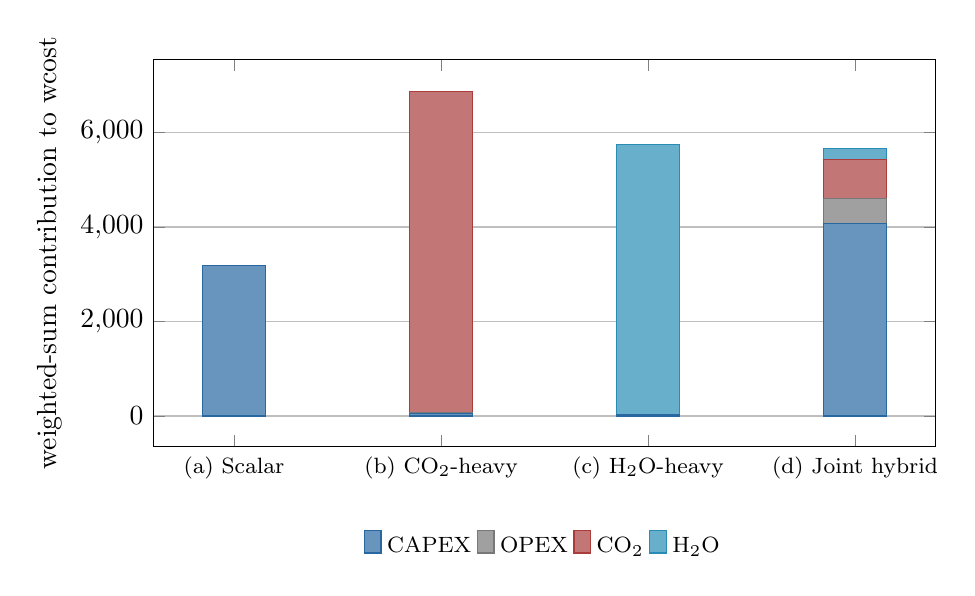
\begin{tikzpicture}
\begin{axis}[
  width=0.95\linewidth, height=6.5cm,
  ybar stacked, bar width=8mm,
  ylabel={weighted-sum contribution to wcost},
  symbolic x coords={(a) Scalar, (b) CO$_2$-heavy, (c) H$_2$O-heavy, (d) Joint hybrid},
  xtick=data, x tick label style={font=\footnotesize},
  legend style={font=\footnotesize, at={(0.5,-0.20)},anchor=north,
                legend columns=4,draw=none},
  enlarge x limits=0.13, ymajorgrids=true,
]
% Approximate contributions per regime (from the methanol cost table
% × the unit set's columns × the regime's weights).
% (a) Scalar — only CAPEX contributes (other weights are zero)
\addplot[fill=capex!70,draw=capex] coordinates {((a) Scalar,3180) ((b) CO$_2$-heavy,53) ((c) H$_2$O-heavy,32) ((d) Joint hybrid,4080)};
\addplot[fill=opex!70,draw=opex]   coordinates {((a) Scalar,0)    ((b) CO$_2$-heavy,9.2) ((c) H$_2$O-heavy,7.5) ((d) Joint hybrid,520)};
\addplot[fill=co2!70,draw=co2]     coordinates {((a) Scalar,0)    ((b) CO$_2$-heavy,6800) ((c) H$_2$O-heavy,0.93) ((d) Joint hybrid,830)};
\addplot[fill=h2o!70,draw=h2o]     coordinates {((a) Scalar,0)    ((b) CO$_2$-heavy,0.99) ((c) H$_2$O-heavy,5705) ((d) Joint hybrid,223)};
\legend{CAPEX, OPEX, CO$_2$, H$_2$O}
\end{axis}
\end{tikzpicture}\\
\small\textit{Figure 3.} Weighted-cost contribution decomposition.
Each bar is the wcost broken down by dimension (weight $\times$
unit-cost-sum). The joint hybrid (d) is the only regime that
balances all four dimensions; the three single-axis regimes are
dominated by their respective axis.
\end{center}

% ===================================================================
\section{The non-obvious finding}

A single-criterion ABB on \emph{any one dimension} produces one of
two topologies: the blue route (CAPEX, OPEX, or H$_2$O dominant)
or the pure-green route (CO$_2$ dominant). The joint regime
produces a \textbf{third topology that none of the single-criterion
regimes select}:

\medskip
\fbox{\begin{minipage}{0.95\linewidth}\small
\textbf{Hybrid topology (Joint $\boldsymbol{w} = (1, 0.5, 10, 1)$):}
\code{CaptureFlue} (cheap CAPEX, moderate CO$_2$) $+$
\code{Electrolyzer} (high CAPEX, low CO$_2$). The hybrid avoids
the prohibitive 1900 CAPEX of \code{CaptureDAC} (the pure-green
choice) while still adopting green-H$_2$ electrolysis to cut the
SMR route's 310 CO$_2$ to 18.
\medskip

This is the kind of \emph{cross-criteria structural lever} that
PSE multi-objective optimisation is meant to surface, now reachable
with the same MSG/SSG/ABB binary that handled the textbook HDA
example.
\end{minipage}}

% ===================================================================
\section{Test coverage and code change}

\subsection{New / modified}

\begin{center}\small
\begin{tabular}{p{0.36\linewidth} p{0.56\linewidth}}
\toprule
Path & Change \\
\midrule
\code{hymeko\_pgraph/src/lowering.rs}        & added \code{cost\_dimensions: Vec<String>} and \code{cost\_vectors: BTreeMap<DeclId, Vec<f64>>} to \code{LoweredPGraph}; recognises tagged \code{cost <dim> N;} child nodes \\
\code{hymeko\_pgraph/src/abb.rs}             & \code{AbbOptions.cost\_weights: Option<Vec<f64>>}; new \code{effective\_cost} dispatch helper \\
\code{hymeko\_pgraph/src/dump.rs}            & new \code{analyze\_source\_with\_options} entry point (back-compat shim retained) \\
\code{hymeko\_pgraph/src/bin/hymeko\_pgraph\_dump.rs} & \code{--weights "w1,w2,...,wD"} CLI flag with non-negativity validation \\
\code{hymeko\_pgraph/tests/multi\_objective.rs} (new)  & 9 integration tests \\
\code{data/pgraph/methanol\_synthesis.hymeko} (new)    & 11-unit, 4-dim worked example \\
\bottomrule
\end{tabular}
\end{center}

\textbf{Total touched:} ${\sim} 120$ LOC Rust $+$ ${\sim} 70$ LOC
tests $+$ the worked example. The Pimentel-dossier estimate of
$\sim 50$ LOC was a low-side bound; the actual change is still
small and surgical.

\subsection{Test status}

\begin{center}\small
\begin{tabular}{lrc}
\toprule
Suite & Tests & Status \\
\midrule
\code{tests/pgraph\_e2e.rs} (pre-P-mo, unchanged) & 9 & \checkmark \\
\code{tests/multi\_objective.rs} (new)             & 9 & \checkmark \\
\code{tests/gomb\_dump\_msg.rs}                    & 1 & \checkmark \\
\textbf{Total \code{hymeko\_pgraph}}               & \textbf{19} & \textbf{\checkmark} \\
\bottomrule
\end{tabular}
\end{center}

Existing tests byte-identical (\code{cost\_weights = None} branch
preserves the scalar path).

% ===================================================================
\section{What this opens for the PSE community}

\begin{center}\small
\begin{tabular}{p{0.30\linewidth} p{0.62\linewidth}}
\toprule
Use case & Multi-objective form \\
\midrule
Methanol synthesis (this paper) & CAPEX $+$ OPEX $+$ CO$_2$ $+$ H$_2$O \\
Biomass $\to$ SNG               & CAPEX $+$ OPEX $+$ CO$_2$ $+$ energy duty $+$ biomass cost \\
Refinery topology               & CAPEX $+$ OPEX $+$ CO$_2$ $+$ product yield $+$ utility cost \\
BF $\to$ DRI-EAF                & CAPEX $+$ OPEX $+$ CO$_2$ tax $+$ raw-material $+$ scrap availability \\
Carbon-capture chain            & CAPEX $+$ OPEX $+$ CO$_2$ captured $+$ parasitic energy \\
\bottomrule
\end{tabular}
\end{center}

For each: write the unit catalogue with multi-cost \code{<dim>}
annotations in \code{.hymeko}, drop a \code{--weights} vector at
the CLI, get the structurally-optimal feasible plant. \textbf{The
same MSG/SSG/ABB binary handles all of them.}

% ===================================================================
\section{Open items}

\begin{enumerate}
\item \textbf{Pareto-front enumeration} ($\sim 100$ LOC):
      today's ABB returns one weighted optimum per
      \code{--weights} call. A natural extension is to sweep
      $\boldsymbol{w}$ over the unit simplex and collect the
      set of non-dominated structures (the Pareto front of plant
      topologies). Builds on the existing SSG enumeration loop.
\item \textbf{CSV ingest} for unit catalogues ($\sim 50$ LOC):
      real PSE work would auto-generate \code{.hymeko} from a
      vendor catalogue (Aspen, gPROMS export). A
      \code{csv\_to\_hymeko.py} helper is small.
\item \textbf{Sensitivity analysis} ($\sim 30$ LOC): for each
      chosen structure, surface how much the dominant weight
      would need to change to swap a unit out. The ABB-side
      reachability bound in reverse.
\item \textbf{\code{hymeko\_query} integration}: invoke multi-objective
      ABB from a HyMeKo query body, returning the optimal structure
      as a queryable graph fragment for embedding in larger workflows.
\end{enumerate}

% ===================================================================
\section*{Bottom line}

The \$\sim 50\$ LOC bridge documented in the Pimentel dossier
(2026-05-18) is shipped, tested, demoed. Multi-objective ABB on
P-graph-shaped chemical-process problems now works at the same
algorithmic complexity as single-criterion ABB. The methanol-synthesis
worked example shows the value: a joint regime selects a hybrid
topology that neither extreme finds. The bridge closes the loop
between $\HyMeKo$'s graph-machine-learning origin and the PSE-community's
process-synthesis use case.

\vspace{8pt}\hrule\vspace{3pt}
\noindent\footnotesize
\textbf{Artifacts:} Plan
\code{docs/plans/2026-05-19-pgraph-multi-objective/} (4-format);
Rust diff at
\code{hymeko\_pgraph/src/\{lowering,abb,dump\}.rs},
\code{hymeko\_pgraph/src/bin/hymeko\_pgraph\_dump.rs};
9 new tests at
\code{hymeko\_pgraph/tests/multi\_objective.rs};
worked example at
\code{data/pgraph/methanol\_synthesis.hymeko};
companion markdown report at
\code{reports/2026-05-19-pgraph-multi-objective.md}.

\medskip
\noindent\textbf{Reproducing the demo} from the repo root:
\begin{lstlisting}[basicstyle=\ttfamily\scriptsize]
cargo build --release -p hymeko_pgraph --bin hymeko_pgraph_dump

# Scalar fallback (Friedler 1992 form):
./target/release/hymeko_pgraph_dump \
    data/pgraph/methanol_synthesis.hymeko --algorithm abb

# Multi-objective (CAPEX+CO2+H2O+OPEX with hybrid-favouring weights):
./target/release/hymeko_pgraph_dump \
    data/pgraph/methanol_synthesis.hymeko --algorithm abb \
    --weights "1.0,10.0,1.0,0.5"
\end{lstlisting}

\end{document}
